\documentclass[a4paper,12pt]{article}

\usepackage{rotating}
\usepackage[top=1in, bottom=1in, left=0.75in, right=0.75in]{geometry}
\usepackage{graphicx}
\usepackage[numbers,square,sort&compress]{natbib}
\usepackage{setspace}
\usepackage[cdot,mediumqspace,]{SIunits}
\usepackage{caption}
\usepackage{subcaption}
\usepackage{mathtools}
\usepackage{authblk}
\usepackage{float}
\renewcommand{\thesubsection}{\thesection.\alph{subsection}}
\providecommand{\e}[1]{\ensuremath{\times 10^{#1}}}

\begin{document}
\onehalfspacing
\title{PHY 407 Lab 9}
\author{Natalie Price-Jones, 999091021}
\date{7 November 2014}
\affil{\small{natalie.price.jones@mail.utoronto.ca}}
\maketitle

\section{Question 1}

\begin{figure}[H]
\centering
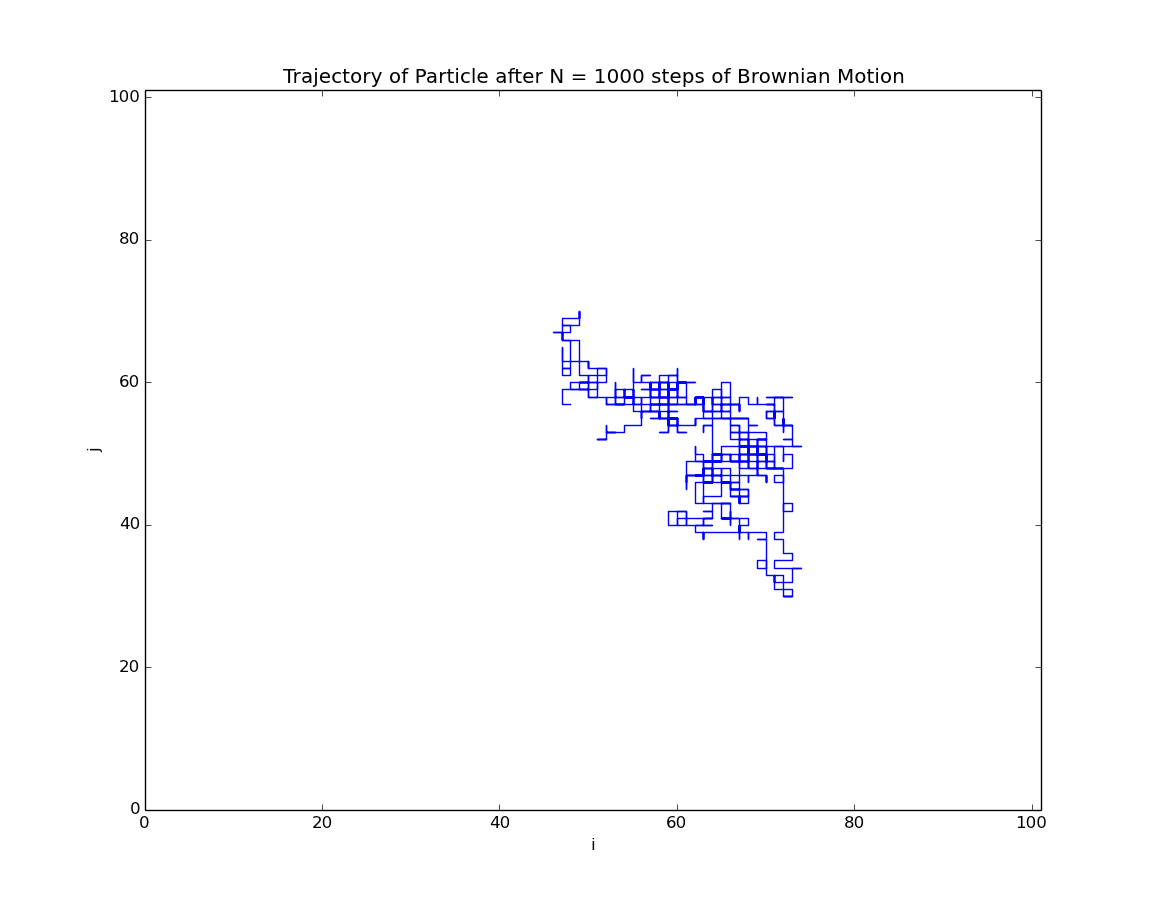
\includegraphics[width = \linewidth]{lab10_q1.png}
\caption{}
\label{fig:q1}
\end{figure}

To demonstrate that my program obeys the rigid wall conditions of the problem, I ran it for more steps to produce Figure \ref{fig:q1aux}. I chose a seed value for the random number generation, so the beginning of the trajectory is the same as Figure \ref{fig:q1}.

\begin{figure}[H]
\centering
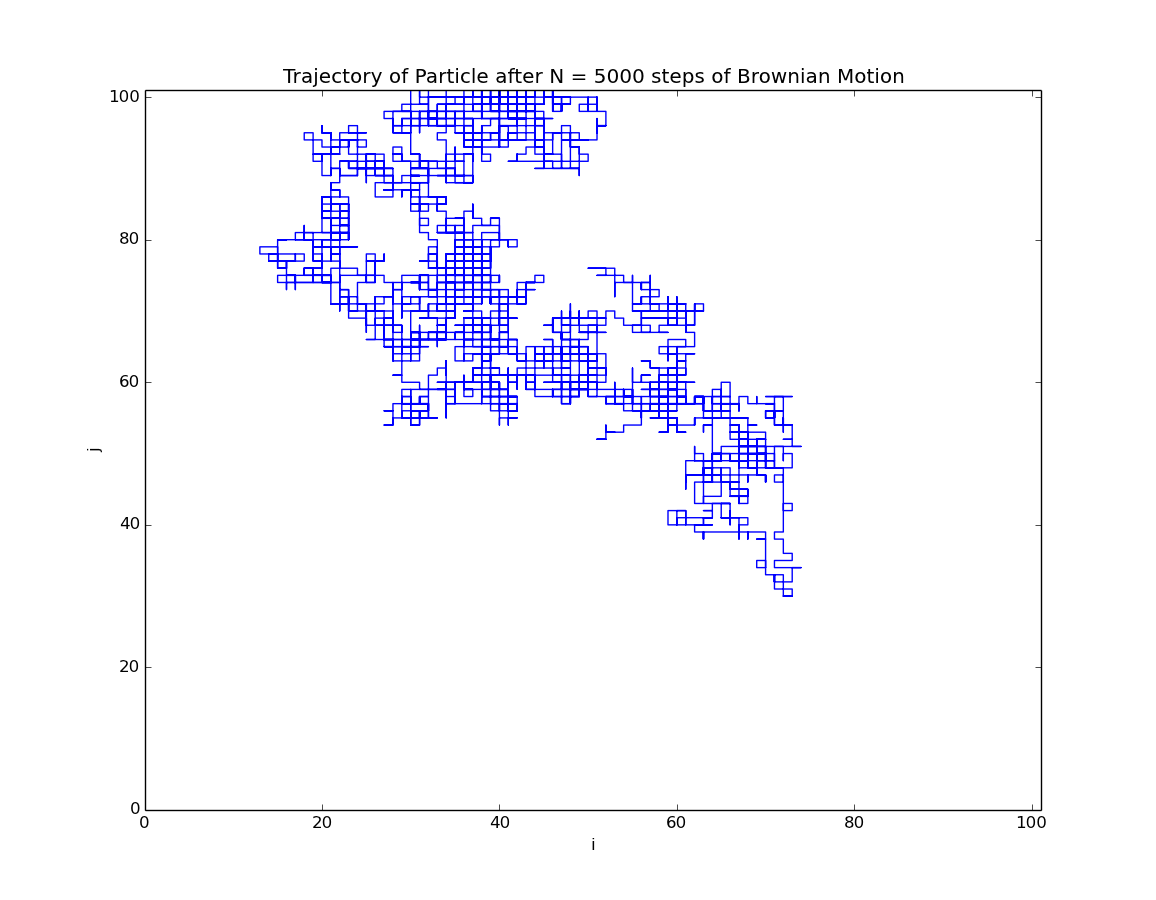
\includegraphics[width = \linewidth]{lab10_q1aux.png}
\caption{}
\label{fig:q1aux}
\end{figure}

\section{Question 3}

\begin{figure}[H]
\centering
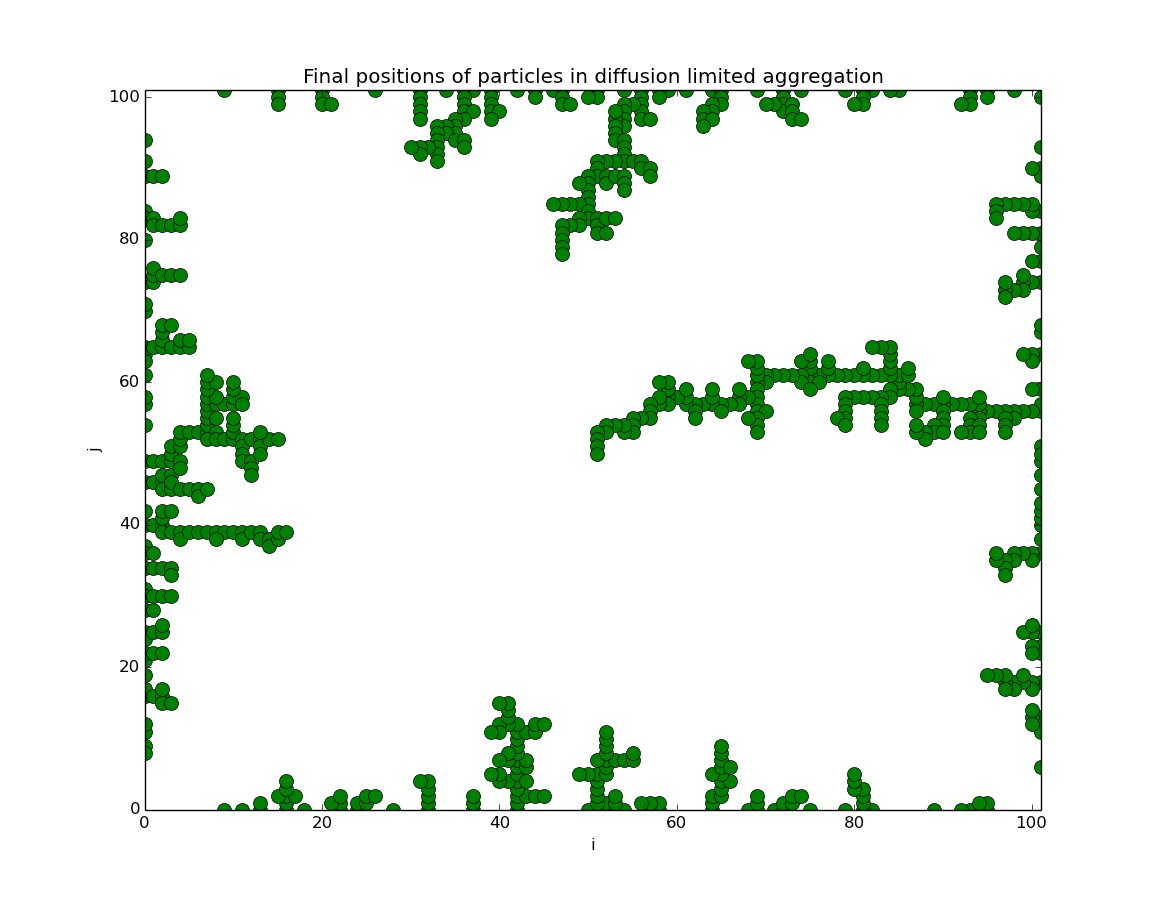
\includegraphics[width = \linewidth]{lab10_q3.png}
\caption{}
\label{fig:q3}
\end{figure}

\section{Question 4}

The volume of a 10 dimensional hypersphere as calculated with the Mean Value Monte Carlo method is $I = 2.56 \pm 0.05$, where the uncertainty was calculated via the following equations:

\begin{eqnarray}
\sigma &=& 2^{n}\sqrt{\frac{\mathrm{var}\,f}{N}},\nonumber\\
\mathrm{var}\, f &=& \langle f^2\rangle - \langle f\rangle^2,\nonumber\\
&=& \frac{1}{N}\sum_{i=1}^N(f(x_i))^2 - \left(\frac{1}{N}\sum_{i=1}^N f(x_i)\right)^2,
\end{eqnarray}
%
where $x_i$ is the $i$th random vector of length $n$ (specifying a point in $n$ dimensional space) and $N$ is the total number of $x_i$'s used to evaluate the integral.  The factor of $2^n$ in the expression for $\sigma$ comes from the fact that our random numbers are drawn from the hyper cube in $n$ dimensions with side length 2. $f(r)$ is a function such that if $\|{(x_i)}\| < R$ (where $R$ is the radius of the hyper sphere) $f(x_i) = 1$, otherwise $f$ returns zero. In this problem, $R = 1$, $n = 10$ and $N = 10^6$.

\section{Question 6}

\begin{figure}[H]
\centering
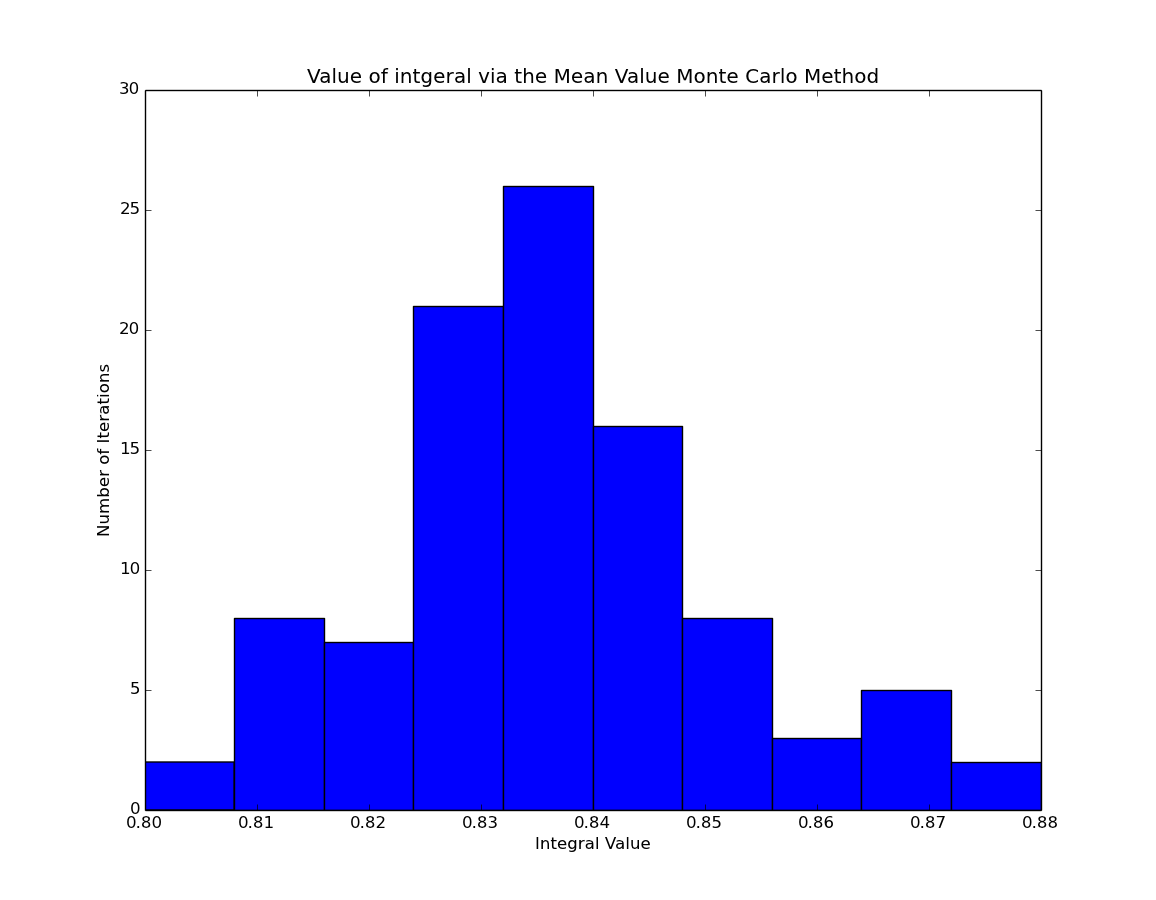
\includegraphics[width = \linewidth]{lab10_q6.png}
\caption{}
\label{fig:q6}
\end{figure}

\section{Question 7}

\begin{figure}[H]
\centering
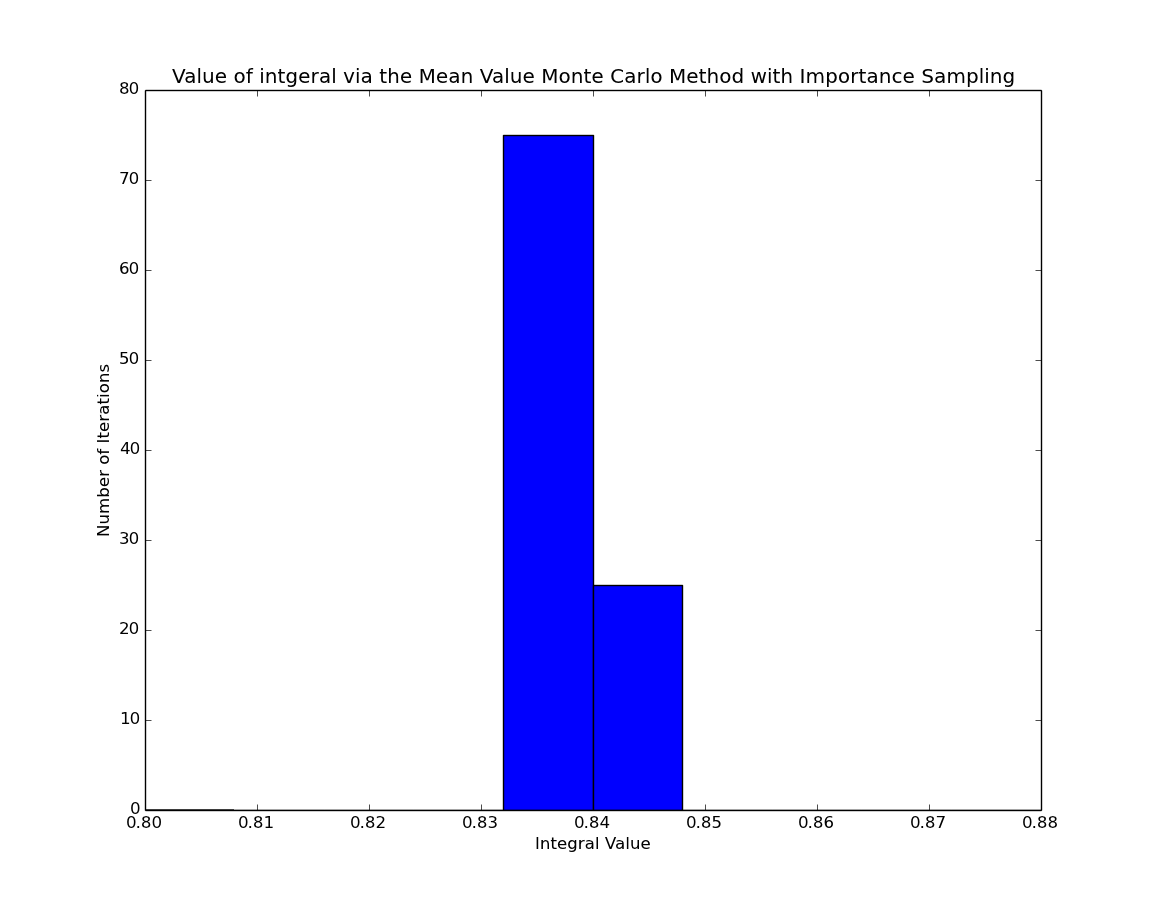
\includegraphics[width = \linewidth]{lab10_q7.png}
\caption{}
\label{fig:q7}
\end{figure}

Obviously the distribution of results in Figure \ref{fig:q7} is much narrower than the one in Figure \ref{fig:q6}. This tells use that importance sampling improves the accuracy of our integral evaluation. This is what we expected - when we use importance sampling, we preferentially take our random numbers farther away from $x = 0$, where our integrand experiences a discontinuity. Near $x = 0$, the values of the integrand are large. The results in Figure \ref{fig:q6} come from uniformly sampled $x$'s in the integration range, which results in some of these very large values being included in the mean value method sum. This causes a larger spread in results, although they still peak in the same bin as Figure \ref{fig:q7}. However since importance sampling avoids these troublesome values, its results are much tighter.

\end{document}